%%%%%%%%%%%%%%%%%%%%%%%%%%%%%%%%%%%%%%%%%%%%%%%%%%%%%%%%%%%%%%%%%%%
%                                                                 %
%                            CHAPTER TWO                          %
%                                                                 %
%%%%%%%%%%%%%%%%%%%%%%%%%%%%%%%%%%%%%%%%%%%%%%%%%%%%%%%%%%%%%%%%%%%

\chapter{PREVIOUS WORK}
%\resetfootnote %this command starts footnote numbering with 1 again.

A number of instances in the literature mentioned previously uses the term versioning and provenance interchangeably.
Mayernik et al. also notice a similar phenomenon although they use the term lineage instead of versioning \cite{MatthewS.Mayernik201312-039}.
The version model introduced by Barkstrom in Figure \ref{NASALevels} to organize NASA's satellite data collection actually refers to a simplified workflow describing the provenance used to produce each level of data \cite{Barkstrom2003}.
The diagram does not compare objects from the same level since changes to contributing components are only used as an indicator for version change.
In actuality, objects have much more complicated development structures than the one dimensional lifespan indicated by the transition from Level 0 data to Level 3.
The PROV Ontology model in Figure \ref{PROVO} outlines more explicit inter-relations between data objects, and it provides a new dimension with which to consider the interactions of data objects.
More specifically, it outlines the explicit process of an agent performing an activity using an entity to produce a new entity.
In the context of the level system, an agent (either a program or individual) performs a "Produce Instantaneous Fields" activity using "L1 Data" to produce "L2 Data."
However, higher level data sets rarely use only one instance of lower level data.
Calibration values may result from daily readings collected from another data set, but the generality of the ontology allows these relationships to be explicitly expressed.
A more realistic provenance graph looks like the one in Figure \ref{ProvGraph} of an ozone indicator in which a Level 3 object results from the interrelation of multiple lower level products.
An interesting observation of note is that Tilmes remarks in 2011 \cite{TILMES2011548}, 
\begin{quotation}
	Consider the relatively common case of the calibration table, which is an input to the L1B process, changing. Even though the version of the L2 or L3 software hasn’t changed, the data files in the whole process have been affected by the change in the calibration.
\end{quotation}
which Barkstrom already observes in 2003 \cite{Barkstrom2003}
\begin{quotation}
	If scientific data production were easy, instruments would
	have stable calibrations and validation activities would discover no need for
	corrections that vary with time. Unfortunately, validation invariably shows that
	instrument calibrations drift and that algorithms need a better physical basis. Within a Data Set, we can think of a Data Set Version as a collection of files in
	a Data Set that have a homogeneous Data Production Strategy. Within a Data
	Set Version, we expect the code producing the files to be stable. We also expect
	that the algorithm input coefficients will be stable as well. The intent of data
	production is to produce data whose uncertainties are statistically similar under
	similar conditions of observation.
\end{quotation}
indicating a basic view that despite eight years in difference, the continuation of software focused versioning resulting in difficulties of data oriented collections.

\begin{figure}
	\centering
	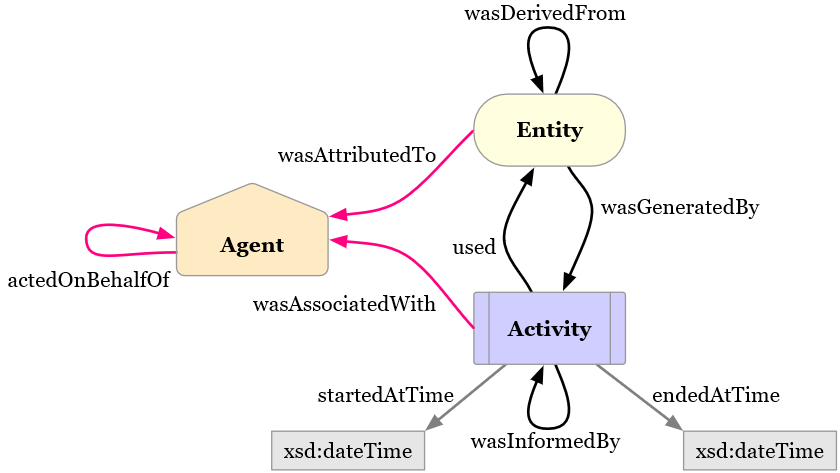
\includegraphics[scale=0.5]{figures/ProvO.png}
	\caption[Diagram of the PROV Ontology.]{Diagram of the PROV Ontology.  Figure 1 from \cite{Lebo2013}}
	\label{PROVO}
\end{figure}

\begin{figure}
	\centering
	\begin{adjustbox}{addcode={\begin{minipage}{\width}}{
					\caption[Provenance graph of a Level 3 data product, showing the inter-relations between different data products in generating the final product.]{Provenance graph of a Level 3 data product, showing the inter-relations between different data products in generating the final product.  Figure 2 from \cite{TILMES2011548}}\end{minipage}},rotate=90,center}
		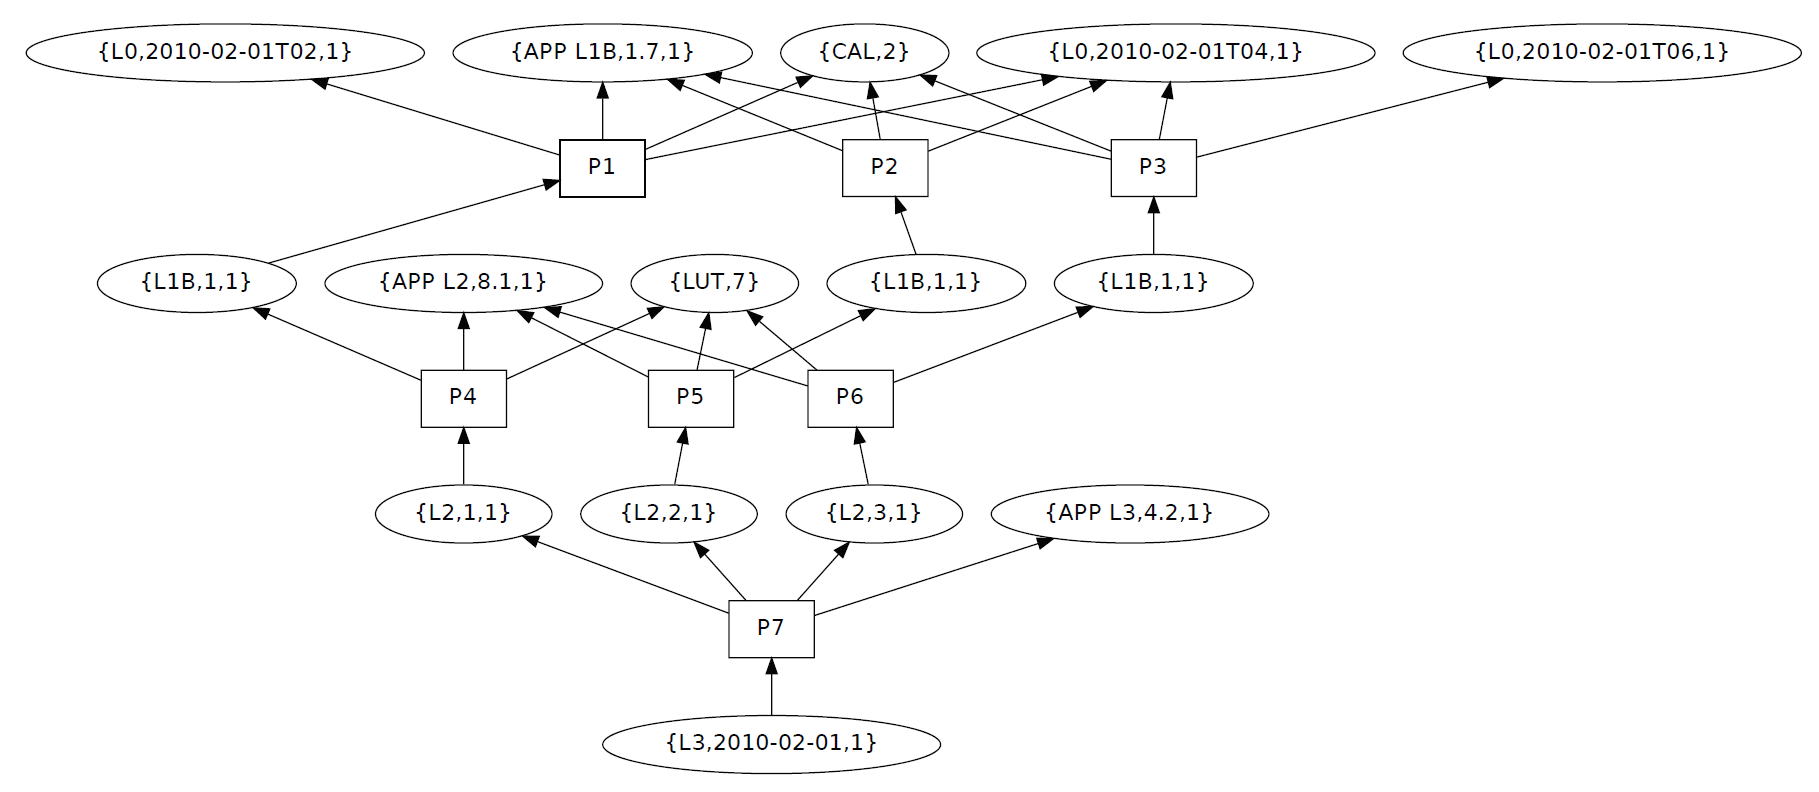
\includegraphics[scale=0.5]{figures/OzoneProvGraph.png}
	\end{adjustbox}
	\label{ProvGraph}
\end{figure}

If the level system provides a length and provenance indicates a breadth of a workflow, a version system can be considered to provide a height to a total workflow.
Referring back to the HCLS data model terminology in Figure \ref{HCLSModel}, as objects within a workflow, as in Figure \ref{ProvGraph}, change versions, the structure of the workflow as well as the Summary Description of the final object, in this case the L3 Ozone product, remains the same.
Instead, the new versions add layers like building blocks over the foundations of the original workflow structure.
Version control systems then provide the mortar linking the blocks together to give the lineage capture procedure a solid structure.

To bring the discussion to an actual application, the GCMD released version 8.4 of their keywords, adding a slew of new values and modifying a select few \cite{Stevens2016}.
At the time of release, many data repositories can be currently assumed to be using the previous or older versions of the keywords.
As the taxonomy is not a class-based ontology, changes to the keywords have significant implications to the semantics of a data set described by those keywords.
A data producer wishing to expose their data sets using the new version of the GCMD Keywords must use a prospective method to translate their current descriptions to the new version.
By comparison, the GCMD would use a retrospective measure to record the changes made to their keywords.
PAV would not be able to address the prospective problem as a result of it is, "a lightweight vocabulary, for capturing “just enough” descriptions essential for web resources representing digitized knowledge" \cite{Ciccarese2013}.
A detailed transition from GCMD Keywords 8.3 to 8.4 would significantly undermine the lightweight nature of the vocabulary.
GCMD does provide a short summary of changes made in a version, but this would come in the form of text rather than structured data.

\section{Provenance}

A number of linked data models include versioning concepts such as the Open Provenance Model (OPM) \cite{moreau2008open}.
Driven by the uncertain needs and sometimes conflicting conventions of different scientific domains, the model sought to find a method to standardize the way in which provenance data is captured while also keeping the specification open to accommodate current data sets through the change.
In an experimental case, the model has been applied to sensor networks, automating and unifying their provenance capture even as they grow \cite{5478496}.
To aid OPM's adoption, the framework Karma2 integrates provenance capture into scientific workflows and provides a more abstract view of their data collection activities \cite{simmhan2010karma2}.
The property WasDerivedFrom constitutes a core concept in the model and marks the reliance of one object's existence on another object.
For a large part, this encompasses the engagement which provenance models view versions, without further need to explore the derivation's content.

PROV, a World Wide Web Consortium (W3C) Recommendation, delineates a method to express data provenance in a more compact form as seen in Figure \ref{PROVO} \cite{Gil2013a} \cite{Groth2013}.
The recommendation uses a conceptual model relating activities, agents, and entities together to describe data production lineage \cite{Moreau2013c} \cite{Nies2013} \cite{Nies2013a}.
Intended as a high level abstraction, it takes an activity oriented approach to provenance modeling.
Every data entity results from the actions of some activity.
The conceptual model's expression occurs through the PROV Ontology (PROV-O), which can be conveyed through various resource description languages \cite{Lebo2013} \cite{Hua2013} \cite{Klyne2013}.
The ontology is further formalized into a functional notation for easier human consumption \cite{Moreau2013b} \cite{Cheney2013a}.
One particular strength that has contributed to the adoption of PROV is its ability to link into other ontologies, making it easier for existing semantically enriched data sets to adopt PROV \cite{Miles2013} \cite{Moreau2013}.
Komadu, a framework developed to alleviate workflow integration, through improves over its predecessor, Karma, by no longer utilizing global context identifiers that were no necessarily shared throughout the workflow. \cite{Suriarachchi_2015}.

The PROV Ontology provides three different concepts that begin to encapsulate the provenance relationship between data versions.
It defines a prov:Generation as "the completion of production of a new entity by an activity," \cite{Lebo2013}.
This means that the generation, which corresponds to the version addition operation, must result from a prov:Activity.
However, activities play a much less active role in versioning since object comparisons instead expose changes.
The property creates a relationship between entities and activities, but such a connection may imply that perturbations in the activity resulted in changing the version.
Changes could also result from modifications in the input data, leading to an entirely new generating activity rather than a modified one.
Prov:Invalidation likewise makes a similar connection between activities and entities.
This means that PROV-O does not have the direct means to communicate the addition and invalidation relationships which exist in our versioning context.
Since we previously establish a state-based view between versions, a more contextually appropriate property should connect two objects together.
Continuing, prov:Derivation does relate two entities and the ontology defines it as, "a transformation of an entity into another, an update of an entity resulting in a new one, or the construction of a new entity based on a preexisting entity. " \cite{Lebo2013}.
In the Marine Biodiversity Virtual Laboratory (MBVL) dataset's case described in Section \ref{sec:MBVL}, none of these three assertions hold true. 
The process simultaneously considers all four versions so one is not transformed into another as would a sequential set of versions.
Additionally, since we do not know which version is the best, we cannot consider any data set as an update of the others.
Finally, no entity preexisted as the data sets resulted from an ongoing analysis and further steps have not been developed.

The PAV Ontology provides a means to track versioning information through linked data by introducing \textit{pav:version} to cite versions and \textit{pav:previousVersion} to link them together in order \cite{Ciccarese2013}.
It does so in comparison to the Dublin Core concept \textit{dc:isVersionOf} which records, "Changes in version imply substantive changes in content rather than differences in format" \cite{DCMI2012}.
PAV argues that a new concept becomes necessary to cover cases where new versions do not have to be substantive but can still be alternate editions of the original object.
Of note is the retrospective nature of the PAV ontology and PROV-O since it places primary emphasis on the most recent edition of an object.
Figure \ref{RCSTree}, shows how RCS stores older versions as back deltas and branches as forward differences.
The retrospective nature of back deltas results from development focus on the latest version, in this case 2.2.
However, the forward differences provide a method to migrate from version 1.3 to the front of the branch.
This characterizes the difference between a focus on data tracking, like that performed by provenance, to data migration, which users must undergo in order to consume the latest version.
Mayernik et al. also find that, "Prospective records document a process that must be followed to generate a given class of products whereas retrospective records document a process that has already been executed" \cite{MatthewS.Mayernik201312-039}.
Retrospective provenance and versioning provides the ability to ensure data trustability and data quality among resources.
However, researchers must follow a prospective versioning record in order to keep their research up to date.

\section{Provenance Distance}

With increasing complexity, data workflows have developed in such a way that even subtle changes have serious implications for other parts of the workflow \cite{TILMES2011548}.
This observation makes change impact difficult to measure, but one insight begins with provenance's role in workflows.
Provenance can give great insight into a data object's future performance such as the  ability to predict disk usage based on the lineage of a data object \cite{dai2014provenance}.
Efforts have also been made to summarize provenance representations to improve consumption \cite{Ainy:2015:ASD:2806416.2806429}.
Changes to the process creating an object signals the development of a new version.
Therefore, studying the magnitude of this deviation should give some idea into the resulting object's impact.
This idea, known as provenance distance, seeks to determine the impact of changes in provenance on new data versions through measuring graph edit distances.

The first ingredient necessary to calculate provenance distance is a linked data graph capturing the sequence of events leading to the old and new objects' creation.
This can be accomplished through the use of previously mentioned provenance models, but these graphs are not widely available.
Using PROV to represent provenance data in a semantic model produces an acyclic directed graph with labeled nodes.
As a result, the provenance distance problem reduces to similarity measurement.
When calculating this measure, algorithms determine how far two graphs are from being isomorphic \cite{Cao2013}.
Node labeling simplifies this process by providing nodes which must match together, and greatly reduces the complexity from computing generalized graphs.
Graph Edit Distance, counting the edits necessary to transform one graph into another, provides a quantitative measure to associate with this process  \cite{Gao2010}.
Some variations count edge changes \cite{Goddard:1996:DGU:246962.246972}.

In Figure \ref{GraphEdit}, the left graph transforms through a move of edge 1 and a rotation of edge 4, resulting in an edit distance of two.
Such changes in a provenance graph would demonstrate a change in dependencies between objects used to generate a final notable product.
Similar results from data with small provenance distance would ensure reproducibility, while large distances signals reinforcing confirmation of a result.
More specifically, scientists should expect similar results from datasets which share a lot of provenance if their conclusions are valid and reproducible.
However, large distances and similar results would indicate that the findings are not limited to a single data source.
This kind of analysis resembles comparison measures employed in determining semantic similarity \cite{Hliaoutakis06informationretrieval}.
The main difference lies in comparing the distance between two concepts within a graph as opposed to the graphs' distances.
Captured impact with these methods rely on the significance of changes to contributing activities towards the new version.

\begin{figure}
	\centering
	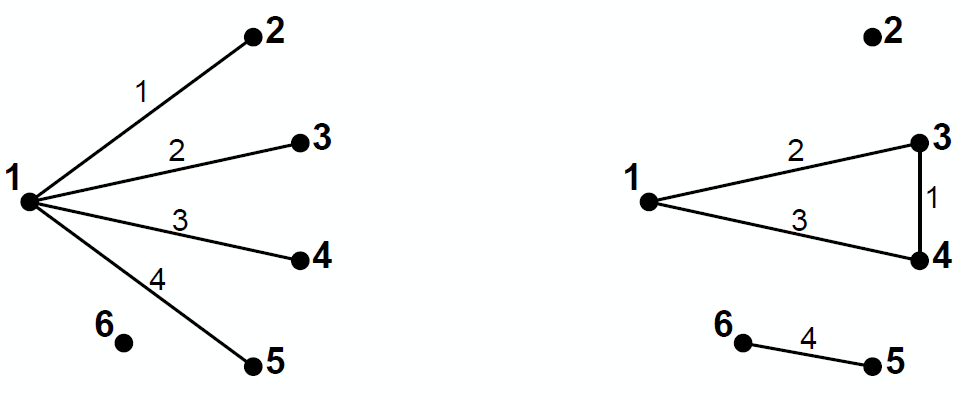
\includegraphics[scale=0.40]{figures/GraphEdit.png}
	\caption[The labeled graph on the left transforms into the right graph under two edge edits.]{The labeled graph on the left transforms into the right graph under two edge edits. Figure 2 from \cite{Goddard:1996:DGU:246962.246972}}
	\label{GraphEdit}
\end{figure}

Methods to provide quality of service boundaries leveraging provenance already exist which compare workflows based on performance criteria \cite{2015:CAA:2778374.2778504}.
However, these procedures focus primarily on quick retrieval and efficient storage instead of capitalizing on the latent information accessed by reasoning across data set versions \cite{tan2004research}.
The distance measures previously mentioned rely solely on provenance graphs to compute results, but this is obviously insufficient.
When considering the provenance of a data object, methods only consider the activities and entities that took an active role in the production of it.
A new version of an object has a familial relationship with its previous versions, but in most cases, they do not take an active role in its generation.
Without detailed change information, determining the difference between two data objects in a metric beyond broad strokes becomes difficult if not impossible.

As per our definition of version, objects must have common provenance, and the more similar they are, versioning methods will have more meaningful results.
Provenance distance provides a means of determining how reliable versioning results are given a greater adoption of provenance graphs.
Measuring a change's impact with accuracy comparable to a change log requires a more detailed understanding and description than provenance can provide  \cite{Bose:2005:LRS:1057977.1057978}.
Sufficiently precise versioning measurements cannot be provided by provenance distance, but it could indicate the confidence of versioning results, which is out of scope for this project.

\section{Mapping}

Data managers primarily use one of two methods to store data versions: snapshots and deltas.
The snapshot method makes periodic copies of the data's current state.
While storing and retrieve these snapshots can be very quick, they consume significant amounts of space to maintain.
The software manager GIT employs this method and Figure \ref{GITFile} demonstrates an example storage space for multiple versions \cite{Chacon:2009:PG:1618548}.
The squares with dotted outlines indicate unmodified files and instead of copying the old object, the system stores a pointer to it instead.
In addition, GIT compresses and separately stores very old versions which are unlikely to be accessed.
This versioning style may not be ideal for larger or often modified data sets as the size requirements will quickly grow unmanageable.

\begin{figure}
	\centering
	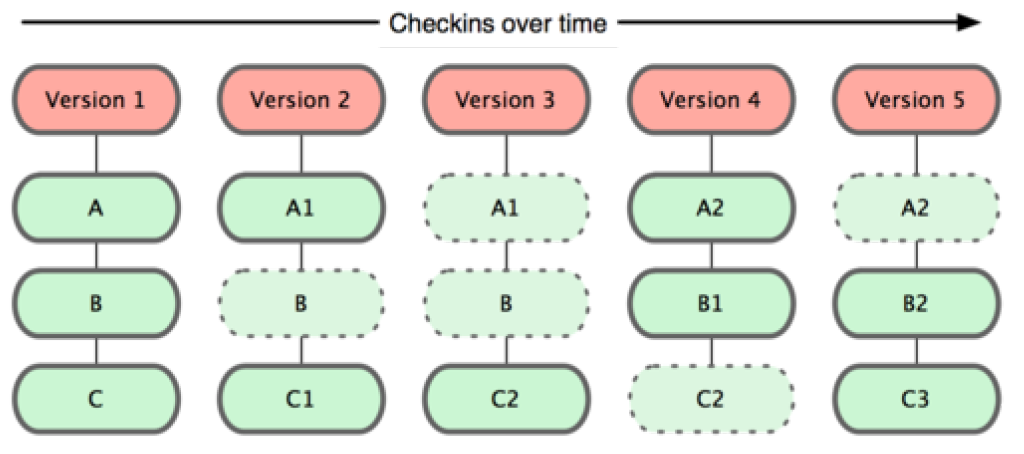
\includegraphics[scale=0.50]{figures/GITFiles.png}
	\caption[GIT stores changes in the repository as snapshots of individual files.]{GIT stores changes in the repository as snapshots of individual files. Figure 1.5 from \cite{Chacon:2009:PG:1618548}}
	\label{GITFile}
\end{figure}

The delta method entails calculating and storing only the differences between one version and the next.
Back delta variations store a snapshot of the most recent version and compute deltas towards older releases.
The forward delta variation stores the oldest data's snapshot and has deltas going forwards.
This method uses the minimum amount of space but trades it in for computation time to recreate any given version.
Properly detecting the addition or modification of a file into a system plays a major role in versioning (ARM)\cite{6906868}.
Ontology Diff \cite{Hartung201315}.



%%% Local Variables:
%%% mode: latex
%%% TeX-master: t
%%% End:
